\section{Boss stage 2: Grunt's playground}

\begin{frame}[fragile]
  \begin{center}
    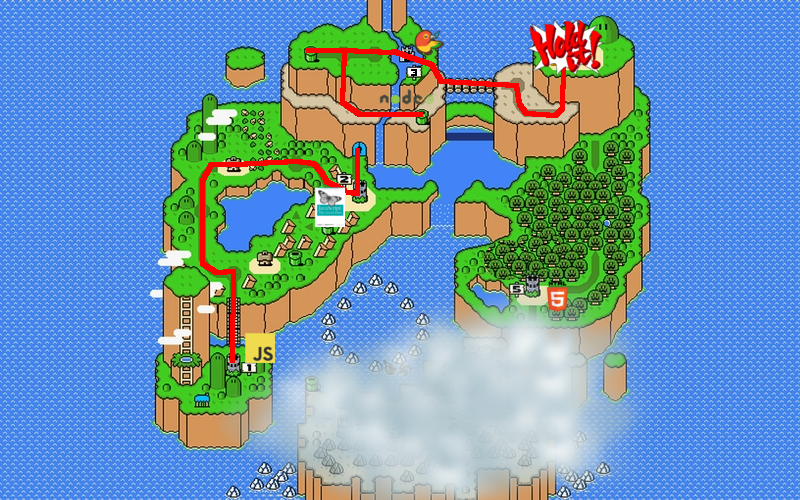
\includegraphics[width=300px]{images/map_boss_stage_2.png}
  \end{center}
\end{frame}

\begin{frame}[fragile]
  \frametitle{Grunt's playground}
  \begin{block}{Exercise}
    \begin{itemize}
      \item Start with the sample code on tag \texttt{boss\_stage\_2}
      \item Remember to install your front-end dependencies using \texttt{bower install}
      \item Remember to install your back-end dependencies using \texttt{bower install}
      \item Run \texttt{grunt watch}
      \item Fix all js lint errors
      \item Add a \texttt{reset.css} and a basic stylesheet to the application
      \item Install \texttt{grunt-contrib-csslint} and \texttt{grunt-contrib-cssmin}
      \item Concat css files and optimize them
      \item Run default task for creating a built and check the result
    \end{itemize}
  \end{block}
\end{frame}
